\problem{Threshold processing}
(a) To make the foreground and background of the image more distinguishable, there are two ways to convert $3$ channels of the image into gray level.
i.e.
\begin{align*}
    I_1 &= \dfrac{1}{3}(R+B+G) \\
    I_2 &= 0.299*R+0.587*B+0.114*G
\end{align*}
The histogram of the intensity of the gray level and its correspondence foreground image is shown in Figure \ref{fig:p2a_result}.\\

\begin{figure}[htbp]
    \centering
    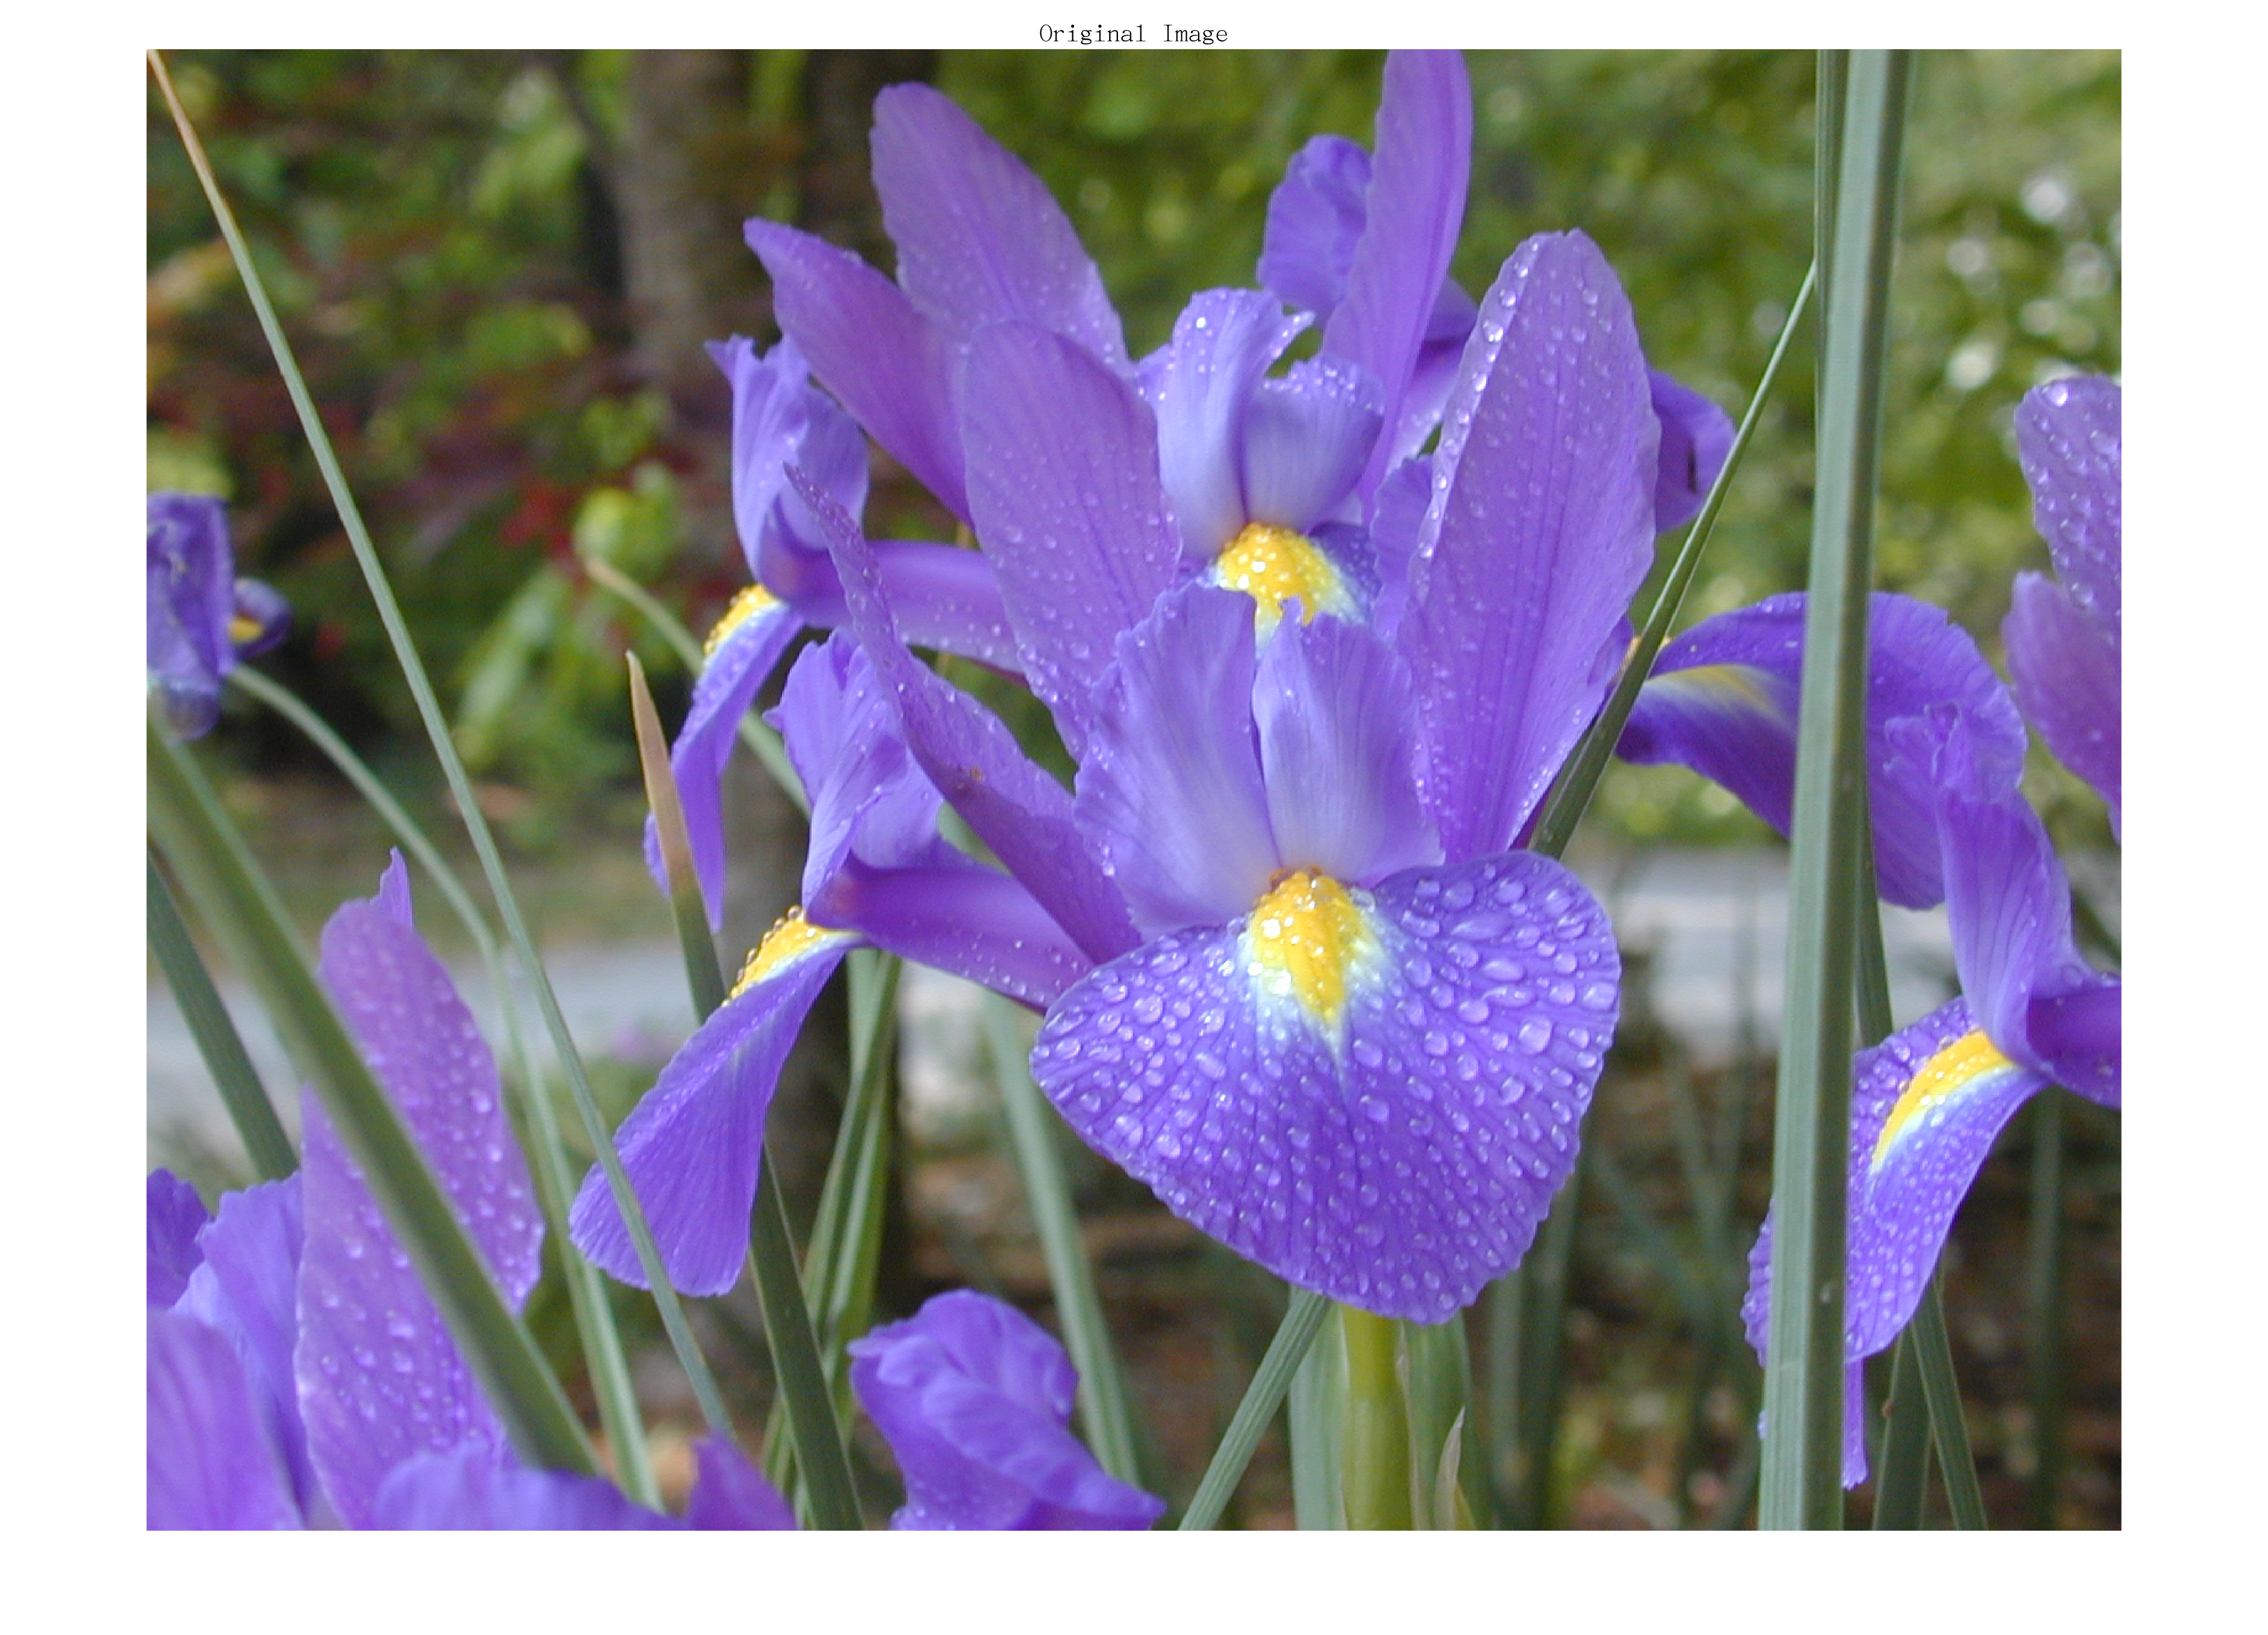
\includegraphics[width=0.4\textwidth]{../images/p2/p2a_origin.png}
    \label{fig:p2a_intensity}
\end{figure}

\begin{figure}[htbp]
\centering
    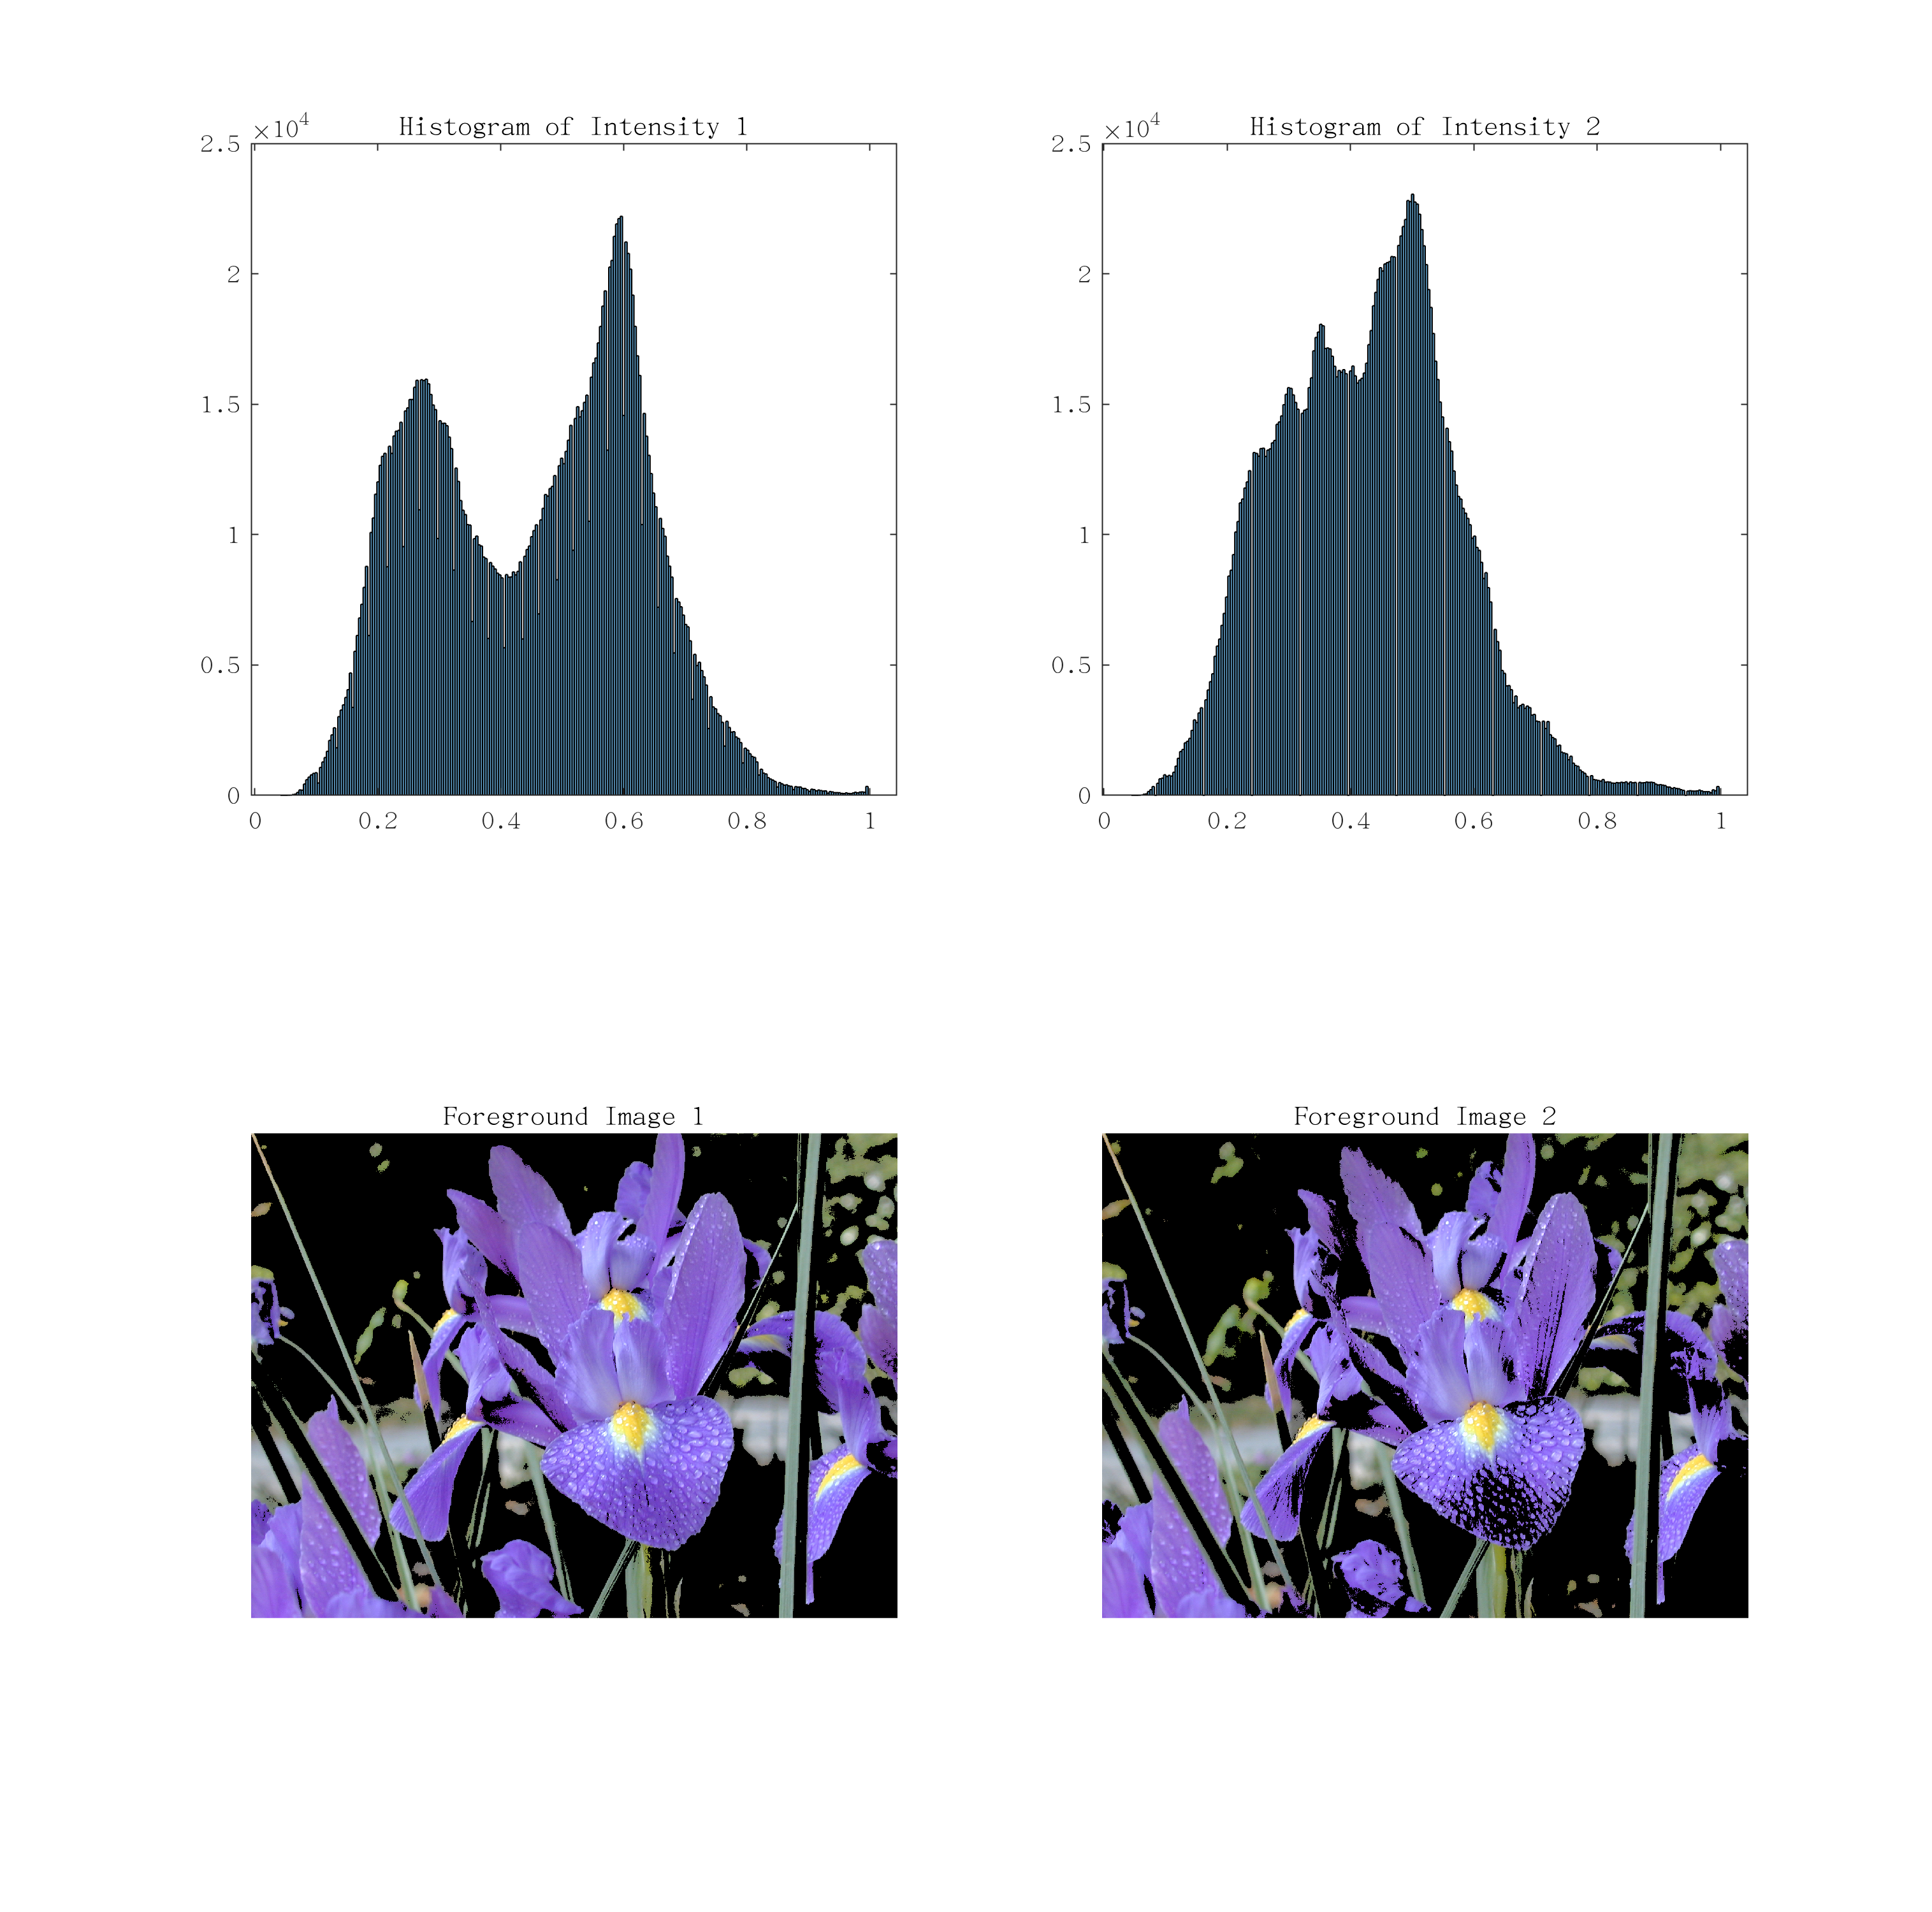
\includegraphics[width=0.75\textwidth]{../images/p2/p2a_result.png}
    \caption{Baisc global thresholding}
    \label{fig:p2a_result}
\end{figure}

(b) The result of Region Splitting and Merging with the minimum four-quadrant size limit of $4*4$ and $8*8$ is shown in Figure \ref{fig:p2b}.\\
The first line is the result of $4*4$ and the second line is the result of $8*8$.\\

\begin{figure}[htbp]
    \centering
	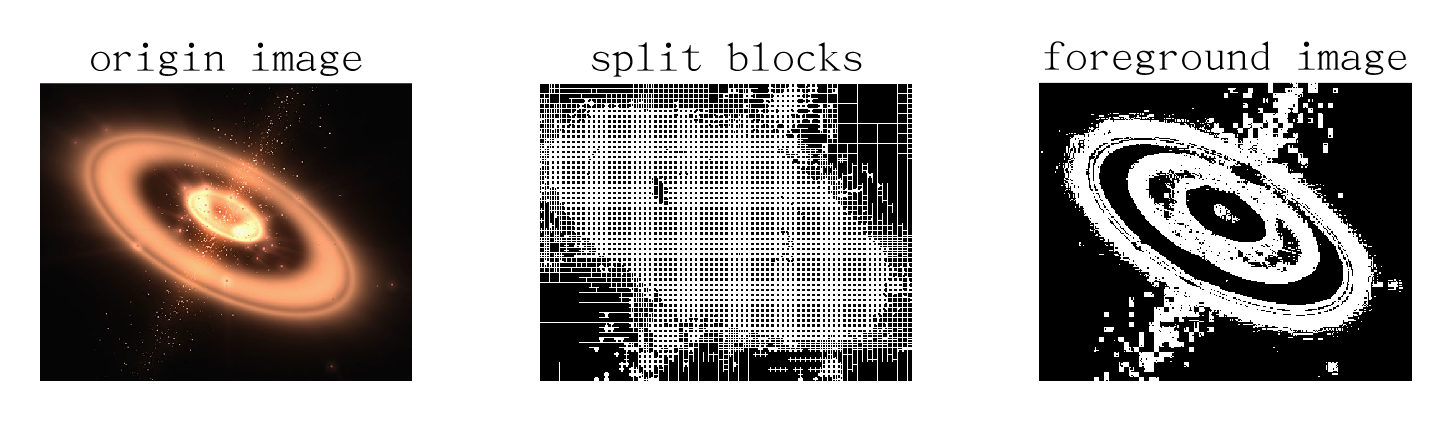
\includegraphics[width=\textwidth]{../images/p2/p2b_blocksize_4.png}
	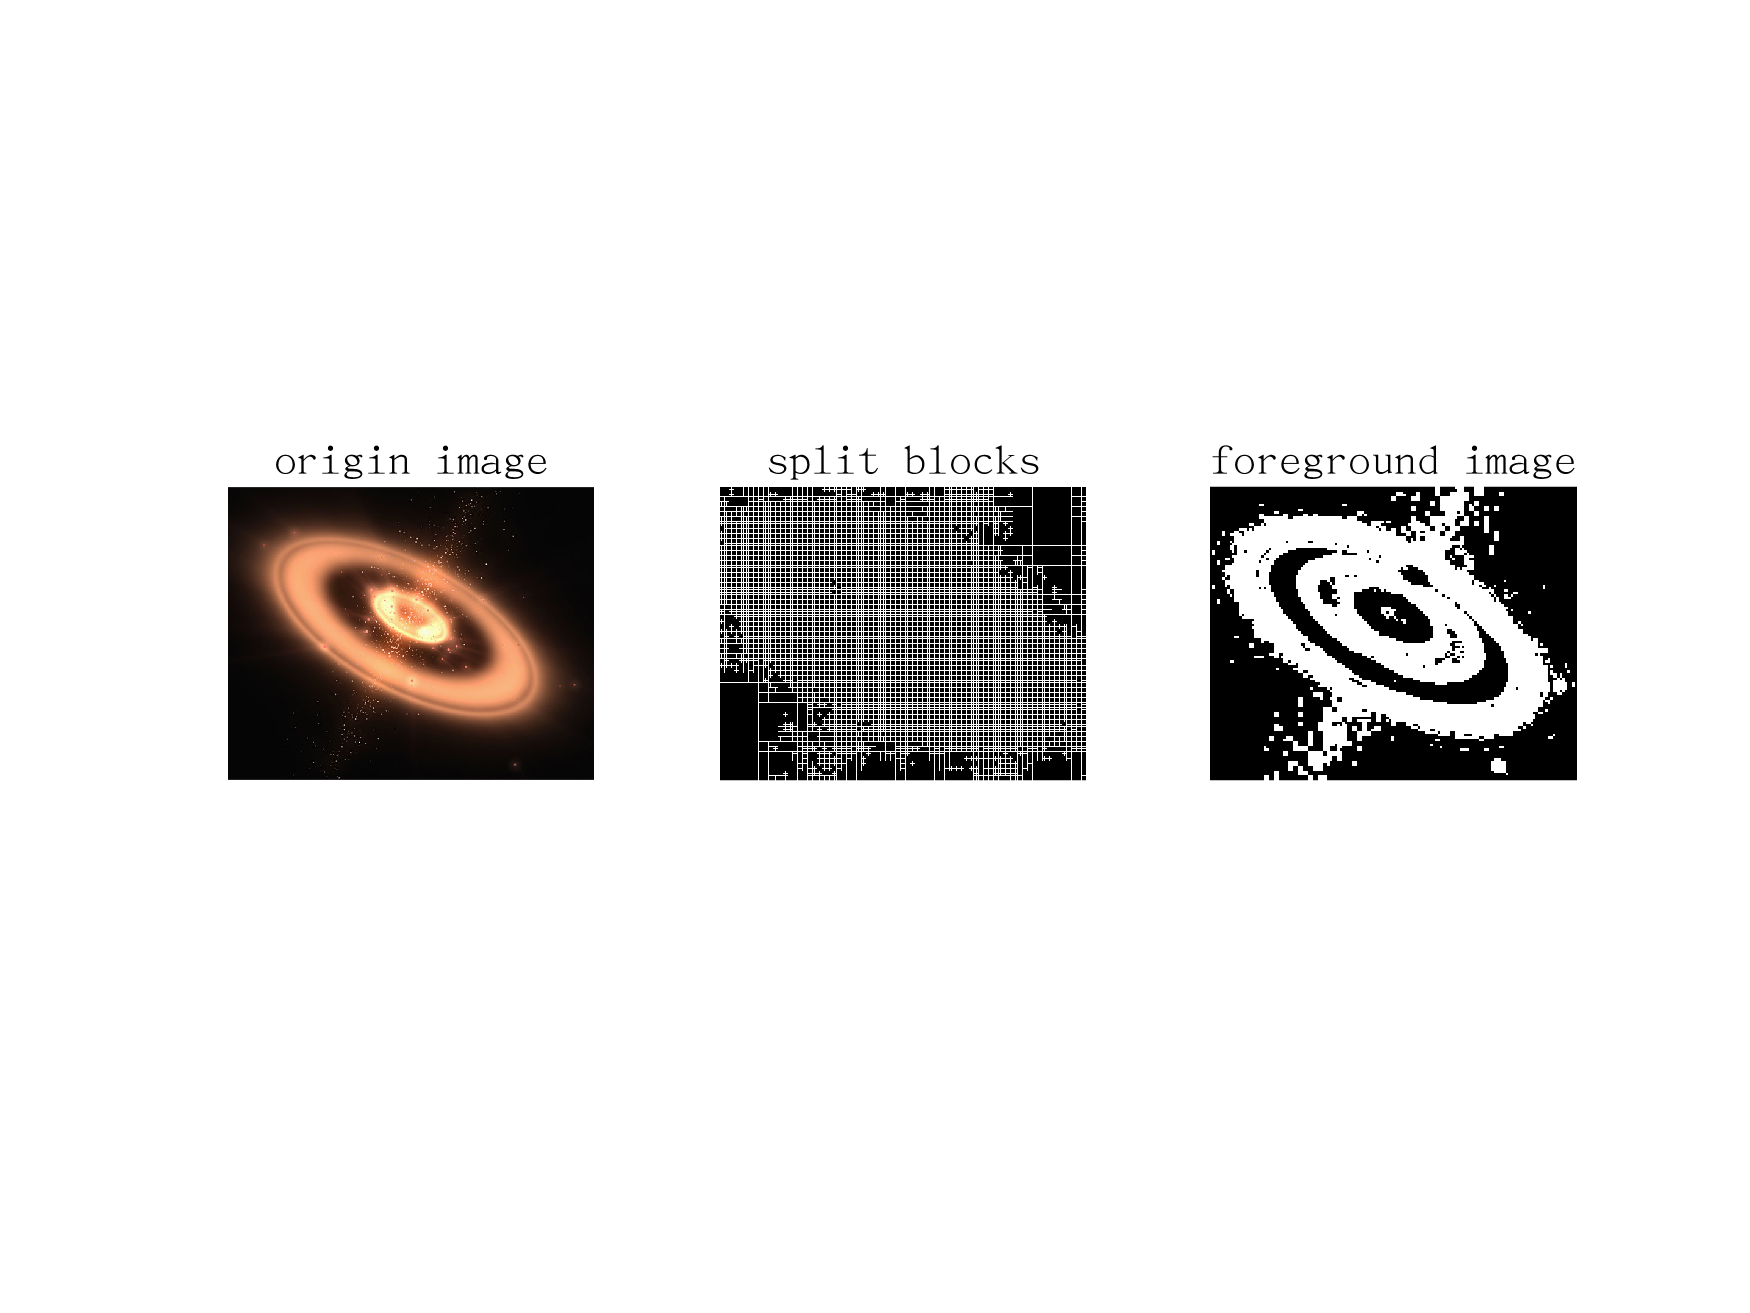
\includegraphics[width=\textwidth]{../images/p2/p2b_blocksize_8.png}
    \caption{Region Splitting and Merging}
    \label{fig:p2b}
\end{figure}

\newpage